\documentclass{article}
\usepackage{tabto}
\usepackage{graphicx}

\title{\textbf{MaSSP AI PROJECT DAILY REPORT NO. 1}}
\author{Team 3}
\date{Monday, July 8th, 2019}


\newcommand{\code}[1]{\texttt{#1}}

\begin{document}
\maketitle
\textit{Project theme: OBJECT DETECTION – Finding certain objects from input images or videos} 
\graphicspath{ {./images/} }

\section{General Progress }
\begin{itemize}
	\item Pinpointed a reliable way to develop this project
	\item Collected a usable training dataset of images online, 12GB of images and annotations from \emph{ \underline{http://cocodataset.org/}}, specfically the 2014 image dataset.
	\item Produced a working code for the AI core of the program (thanks to the help of mentor Giang), using the pre-trained model YOLOv3, specifically the YOLOv3-tiny weights set. (details in section 4.1)
	\item Tweaked the code in order to specifically find one desirable category of item in the image, instead of everything findable. (details in section 4.1)
\end{itemize}


\section{Future Plan}

\begin{itemize}
	\item Deciding on what front-end development path will be used as the wrapper for the AI Core (the votes are leaned to creating an Android application)
	\begin{itemize}
		\item Tools considering to use for Android Application: Kivi (\emph{\underline{https://kivy.org}})
		\item Will make use of the pre-made code from the Facebook group if choose to create a desktop application instead
	\end{itemize}
	\item Probably re-training the model with a specific category in mind
	\item Thinking of analyzing camera in realtime, but the analyzing speed is not quite guaranteed to make an application out of it.
\end{itemize}

\section{Obstacles}
\begin{itemize}
	\item Problem with the possibility of continuing to train the pre-trained model: no idea where to start	
	\begin{itemize}
		\item Already inquired mentors about it, the problem with the solution is that we have to ourseves cherry-picked the layers from the YOLO model to retrain it 
	\end{itemize}
\end{itemize}

\section{Demo}

The Colab link containing the progress so far: \emph{\underline{https://drive.google.com/open?id=}}\\
\emph{\underline{186OWo8ZU0dRYfMjsqumBpMVNRWlR2kwh}}

\subsection{Code Analysis}
\tab \textbf{Summary}: The output images contain every “Pizza” item that is found by the model from the input image, each bounded by a green bounding box. The images are produced chronologically as the bounding boxes are plotted.
	
\begin{itemize}
	\item Input image:\\\\ \centerline{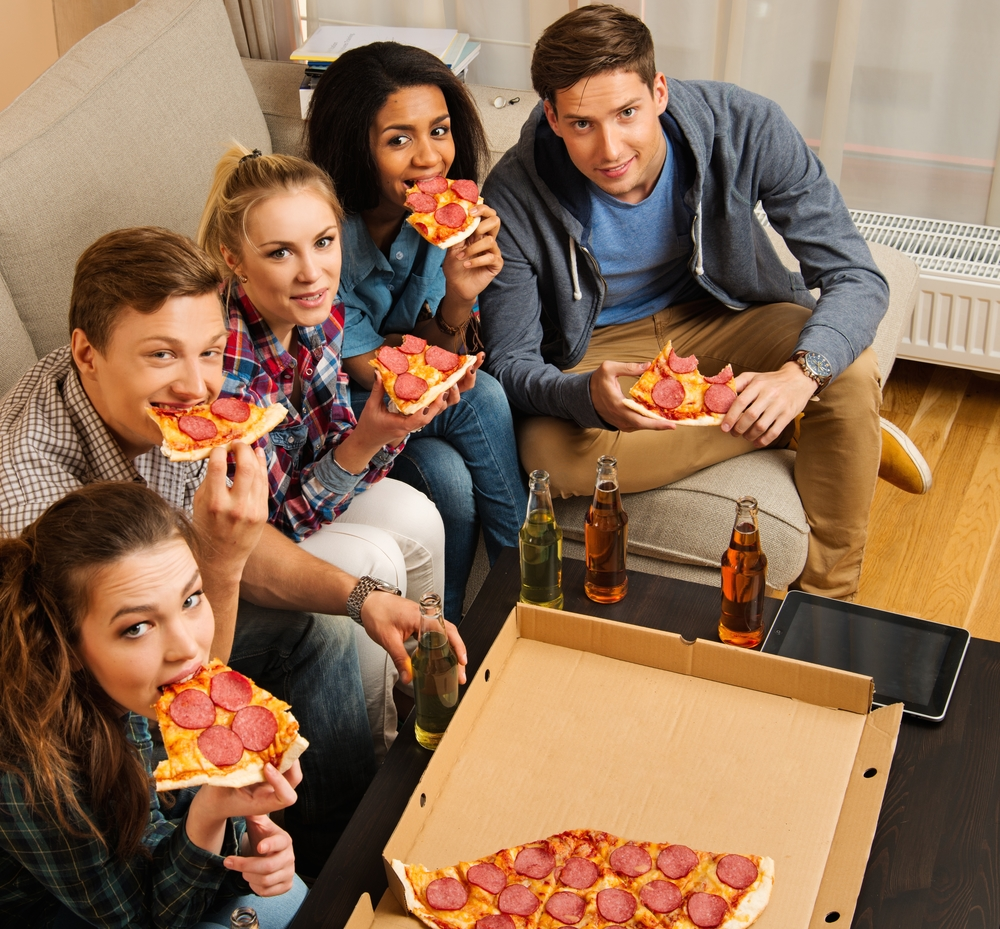
\includegraphics[scale=1]{img12}} \\
	\centerline{\small{\textbf{Image 1: Input image. Resolution 1000 x 929. Source: Internet}}}
	\item Output picture:\\
	\centerline{\includegraphics[scale=1]{img14}}\\
	\centerline{\small{\textbf{Image 2: Output image. The "Pizza" items are identified and pinpointed in the bounding boxes.}}}
	\item Due to the tininess of the yolo-tiny weight, although the analyzing speed is fast, the YOLO-tiny model did not capture every "Pizza" items in the image.
	\item Can set what item category to find in the image by changing the \code{desired\_classes} variable.\\
	\centerline{\includegraphics[scale=1]{img15}}\\
	\centerline{\small{\textbf{Image 3: \code{desired\_classes} responsible for finding specific item}}}
	\item Should the user want to find, say, "Person" category inside the image, he/she can do it by changing \code{desired\_classes} to \code{1}. The output image afte the change:\\
	\centerline{\includegraphics[scale=1]{img16}}\\
	\centerline{\small{\textbf{Image 4: Output image of "Person" items founded in the image}}}
	\item
\end{itemize}
	
\end{document}		